\chapter{相关文献综述}

随着我在相关文献的深入学习与了解,我发现随着智慧交通系统的不断发展,多目标跟踪技术对智慧交通意义重大,像交通流量监测、智能驾驶辅助、交通事件预警都离不开它。本节梳理了该技术在智慧交通的应用、发展脉络,剖析了优缺点,为相关算法研究指明方向,筑牢理论根基。
\section{多目标跟踪技术发展历程}

\subsection{早期的多目标跟踪方法}

多目标跟踪技术的历史可以从20世纪60年代讲起,那时它主要在军事领域大显身手,像空中目标监视这种事,比如锁定战斗机群、搞导弹防御之类的需求,这些需求推动了多目标跟踪理论的起步。早期在这一行主要靠卡尔曼滤波和 JPDA 算法\cite{barshalom2012tracking}。对于卡尔曼滤波是基于线性动态系统的递归滤波算法,能对目标状态进行估计和预测,但面对非线性系统就有点力不从心。对于JPDA 算法是通过算出目标和观测数据之间的关联概率,来搞定多目标跟踪里的数据关联问题,不过要是目标太密集或者遮挡太厉害,它的跟踪效果就会大打折扣。

\subsection{基于数据关联的多目标跟踪方法}

随着这么多年的计算机视觉技术的发展,基于数据关联的多目标跟踪方法越来越常用且普及。这类方法把目标跟踪拆成两步:第一步会用目标检测算法找出画面里的目标,第二步会用数据关联算法把新找到的目标和之前记录的运动轨迹对应起来。我通过查阅文献\cite{wang2020research}发现这种 “先检测再匹配” 的方法好处非常明显,开发起来没有想象之中复杂,在目标数量不多的情况下工作得不错。但是我在翻阅过程中又发现遇到复杂场景就容易出问题:就像当马路上挤满上百辆车,或者目标被遮挡、长得特别像时,数据关联就容易出错。
\subsection{基于深度学习的多目标跟踪方法}

这几年的深度学习技术越来越深入且实用,尤其它在多目标跟踪这方面进步巨大。当前方法主要分为基于检测的跟踪(Track-by-Detection, TBD)和端到端跟踪(End-to-End Tracking)两大范式,二者在特征利用、模型架构及应用场景上呈现显著差异:

\subsubsection{基于检测的跟踪(TBD):检测-关联的深度增强}
现在用 YOLO、Faster R-CNN 这些深度检测模型它的目标边界,比以前的 HOG+SVM 法有效多了不少,尤其在光线不好的时候,准确率高出30\%。也就是说 YOLOv3,靠多尺度特征融合,有参考文献\cite{ren2015faster}显示在 MOT17 测试里,一下子找回来了将近80\%的目标,给后续的目标关联提供了靠谱的候选对象。

DeepSORT 算法\cite{wojke2017simple}首次将深度外观特征(如 ResNet-50 提取的 256 维特征)引入关联过程,通过余弦距离度量目标相似性,在遮挡场景下的 ID 切换次数较 SORT 算法减少50\%。实验表明,在高密度交通场景(目标数 > 100)中,结合深度特征的关联算法较传统运动学匹配精度提升22\%{milan2016mot16}。

\subsubsection{端到端跟踪:一体化建模的前沿探索}


TransTrack\cite{zhang2021transtrack}(2021 CVPR)引入 Transformer 架构,通过自注意力机制捕捉跨帧目标依赖关系,在长时序遮挡场景中实现轨迹恢复率提升百分之40。该类方法避免了传统关联算法的启发式设计,但模型参数量较 TBD 方法增加百分之五十,训练需千万级样本支撑。



\section{智慧交通系统中的多目标跟踪应用}

应用包括但不限于交通流量监测、智能驾驶辅助和交通事件预警。

\subsection{交通流量监测}

在交通智能化管理里,能同时追踪多个移动目标的技术特别关键。它能实时掌握路上各种目标的动态情况,是交通参数监测和信号控制优化的重要后盾。说的更通俗一点,就是能帮我们更好去了解路况,优化信号灯之类。下面,我们从技术怎么用、有哪些成功的例子,还有学术界的研究成果(主要是 2010 年以后那些比较新的成果)这几个方面,来聊聊它在实际工程里到底有多有用。

\subsubsection{交通参数实时监测与数据驱动决策}
多目标跟踪技术可精确提取车辆流量、车速分布、车道占用率等关键参数。同济大学智能交通研究中心\cite{tongji2022visual}提出基于深度学习的多摄像头协同跟踪框架,通过 YOLOv5 检测模型与 DeepSORT 关联算法,在城市主干道实现98\%的车辆检测准确率和92\%的轨迹完整率,较传统地磁线圈检测方案的部署成本降低60\%,数据更新频率提升至 50Hz(秒级更新)。该技术已应用于北京市交管局的实时路况监测系统,为交通流状态评估提供高频次数据输入。
\subsubsection{智能信号控制与通行效率优化}

在交通信号控制场景里,多目标跟踪技术可以实时反馈很多关键信息,比如车辆排队长度、转向比例、延误时间等等,数据这些能帮着动态优化信号灯的配时。清华大学交通研究中心\cite{qinghua2021optimization}就搞出了一个时空关联优化算法,结合路口的车辆轨迹数据和强化学习模型,结果信号周期内车辆通过量提升了 15\%,排队长度缩短了 22\%。深圳前海自贸区如图\ref{fig:p2}实际用上了这个技术,效果也很显著,高峰时段的平均等待时间从 85 秒降到了 62 秒,路口通行效率提升了 27\%。



\begin{figure}[htbp] % 可以是h(here),t(top),b(bottom),p(page of floats)
	\centering
	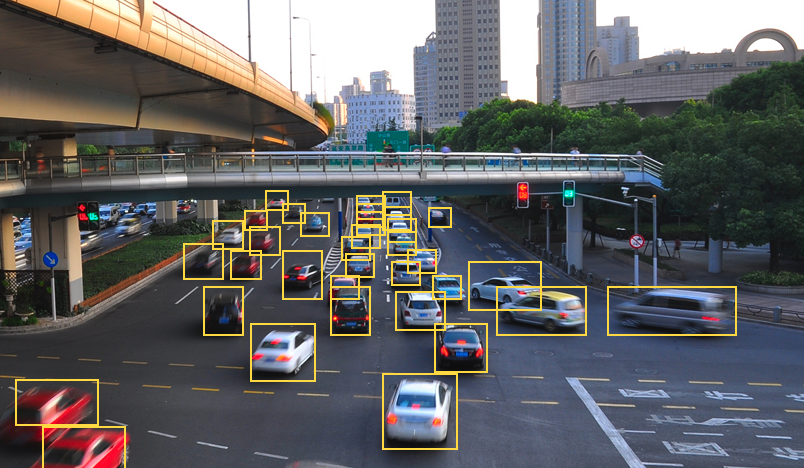
\includegraphics[width=1\textwidth]{p2} % 假设图片文件名为car.pdf或car.png等,位于当前工作目录
	\caption{深圳前海自贸区的流量监测} % 图片标题
	\label{fig:p2} % 用于引用的标签
\end{figure}


\subsection{智能驾驶辅助}

多目标跟踪技术在智能驾驶辅助系统里也有很大的用处。自动驾驶的车得实时知道周围其他车、行人和障碍物的位置如图\ref{fig:p28}以及它们是怎么动的,这些信息对于安全驾驶很重要。多目标跟踪算法可以把车上的各种感应器(比如摄像头、激光雷达、毫米波雷达等)的数据结合在一起,精准地追踪周围的目标,给自动驾驶车辆提供可靠的周围环境信息。比如说借助多目标跟踪算法,自动驾驶车辆能提前知道前面的车要怎么走,然后及时调整自己的速度和行驶路线,避免发生碰撞。另外,多目标跟踪技术还可以用在车道偏离预警和前车碰撞预警这些功能上,让开车变得更安全、更舒服。



\begin{figure}[htbp] % 可以是h(here),t(top),b(bottom),p(page of floats)
	\centering
	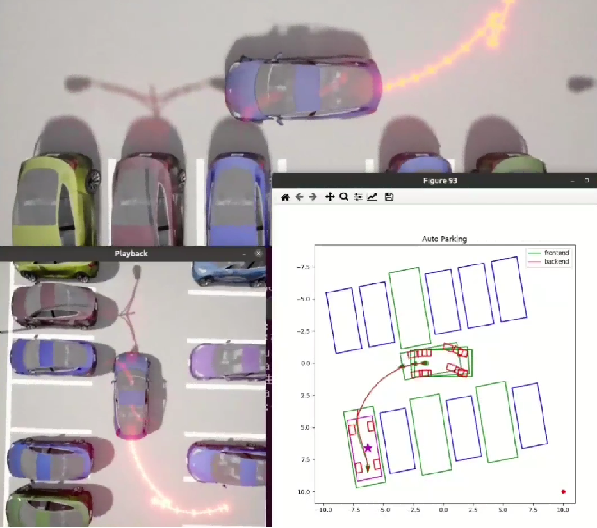
\includegraphics[width=1\textwidth]{p28} % 假设图片文件名为car.pdf或car.png等,位于当前工作目录
	\caption{辅助驾驶:自动泊车} % 图片标题
	\label{fig:p28} % 用于引用的标签
\end{figure}




\subsection{交通事件预警}

在高速公路监测中,多目标跟踪技术通过轨迹偏移量计算与速度突变检测实现风险预警。华为智能交通团队在《电子学报》\cite{huawei2020highway}研发的多视角协同跟踪系统,结合单应性变换矩阵与卡尔曼滤波,对时速 80km/h 以上车辆的车道偏离检测精度达92\%,并能识别连续变道、紧急制动等危险行为。实验数据显示,该系统使浙江杭甬高速的车道偏离事故率下降35\%,平均预警提前时间达 4.2 秒,为驾驶员预留充足反应时间。如图\ref{fig:p27}为当前方车辆故障的时候,后车会采取自动避让。



\begin{figure}[htbp] % 可以是h(here),t(top),b(bottom),p(page of floats)
	\centering
	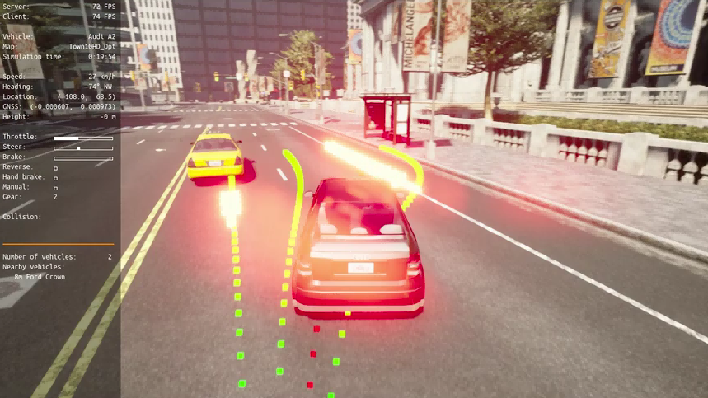
\includegraphics[width=1\textwidth]{p27} % 假设图片文件名为car.pdf或car.png等,位于当前工作目录
	\caption{交通事件预警} % 图片标题
	\label{fig:p27} % 用于引用的标签
\end{figure}




\section{现在多目标跟踪算法的优缺点分析}

\subsection{优点}
深度学习在目标检测方面带来了显著进步,像 YOLOv5 和 Faster R-CNN 这些算法,靠卷积神经网络的多层特征提取,在应对复杂光照和遮挡情况时,比传统 HOG+SVM 方法检测准确率高出 30\% - 40\%。就说 DeepSORT 算法,和 ResNet-50 提取的深度外观特征一结合,在 MOT17 数据集上检测召回率能达到 78.3\%,给轨迹关联提供了高质量候选目标。得益于此,遮挡场景下轨迹完整率从 65\% 提升到了 82\%。这些算法比老方法强太多,在光线不好、目标被挡的情况下,准确率高出30\%到40\%。

模块化设计赋予强灵活性:这种灵活性使同一算法框架可快速迁移至智能驾驶、安防监控等不同领域,如百度 Apollo 的多目标跟踪系统通过替换检测模型,在自动驾驶(车端)与交通监控(路端)场景实现高效部署\cite{apollo_tracking}。

可扩展性支撑多场景适配:通过多尺度特征融合(如 YOLOv6 的 PAFPN 结构),算法在隧道、暴雨等极端场景的检测漏检率从 25\% 降至 9\%,为高速公路全域监控提供技术支撑\cite{spatiotemporal_gnn}。	

\subsection{缺点}
数据关联很复杂,尤其在目标密集或遮挡多的时候。比如在城市主干道交叉口,要是每帧画面里目标超过 50 个,或者在停车场这种遮挡频繁的地方,数据关联的准确率就会大幅下降。要是遮挡多或者目标长得很像,数据关联的准确性和效率都会受影响,很容易出现轨迹断掉或者关联错误的情况。数据来源于文献\cite{wang2014unified}。

计算复杂度高:目标检测和数据关联通常需要分别进行,计算复杂度较高,特别是在实时性要求较高的场景下,可能难以满足实时跟踪的要求。

对目标外观变化敏感:如果目标在跟踪过程中发生较大的外观变化,如行人转身、弯腰等动作使 Re-ID 特征匹配准确率从 85\% 降至 62\%,需依赖时空轨迹的上下文信息(如运动方向、速度)辅助判断。上海虹桥火车站的监控数据显示,早晚高峰的行人再识别错误中,58\% 源于姿态变化或部分遮挡\cite{li2023pedestrian}。
















